\chapter{Results \& Discussion}
All time measurements are in milliseconds (ms,) and are taken as an average over 500 frames and I double check the result. All external applications were closed to maintain result validity between tests. All tests were done on a resolution of 1280*720 on the following system:\\
CPU: Core i7-920 at 2.66GHz\\
RAM: 18GB DDR3\\
GPU: NVIDIA GTX 480\\

I use three different models to test and compare:

\begin{tabular}{| l | r |}
\hline
Scene & Triangles \\
\hline
\emph{Conference} &  331,179 \\
\hline
\emph{Cornell Box} & 35 \\
\hline
\emph{Dragon} &  871,306\\
\hline
\end{tabular}

\section{Deep G-buffer Generation}
I will use the Dragon model to demonstrate the results of the deep g-buffer generation. I have chosen this model specifically because it is a single model with a lot of triangles eliminating the overhead caused by state changes from multiple meshes, while having a high enough triangles to produce reliable rasterising times. Table \ref{table-buffers} shows the resulting normal and depth buffers from generating the G-buffer.

\begin{table}[!ht]
\centering
\begin{tabular}{| c | c | c |}
\hline
Buffer & Layer 1 Result & Layer 2 Result \\
\hline
\emph{Depths} &
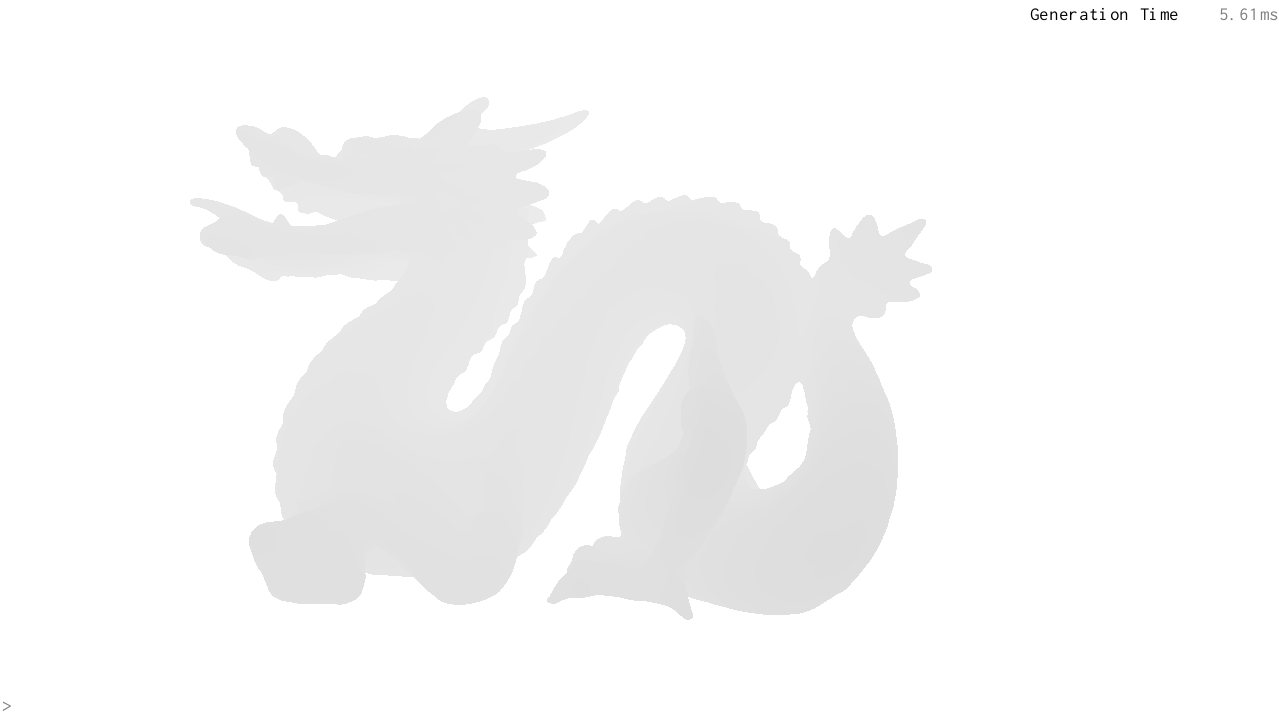
\includegraphics[scale=0.1,trim=0 0 0 -5]{img/results/g-buffer/depths-2layer-1} &
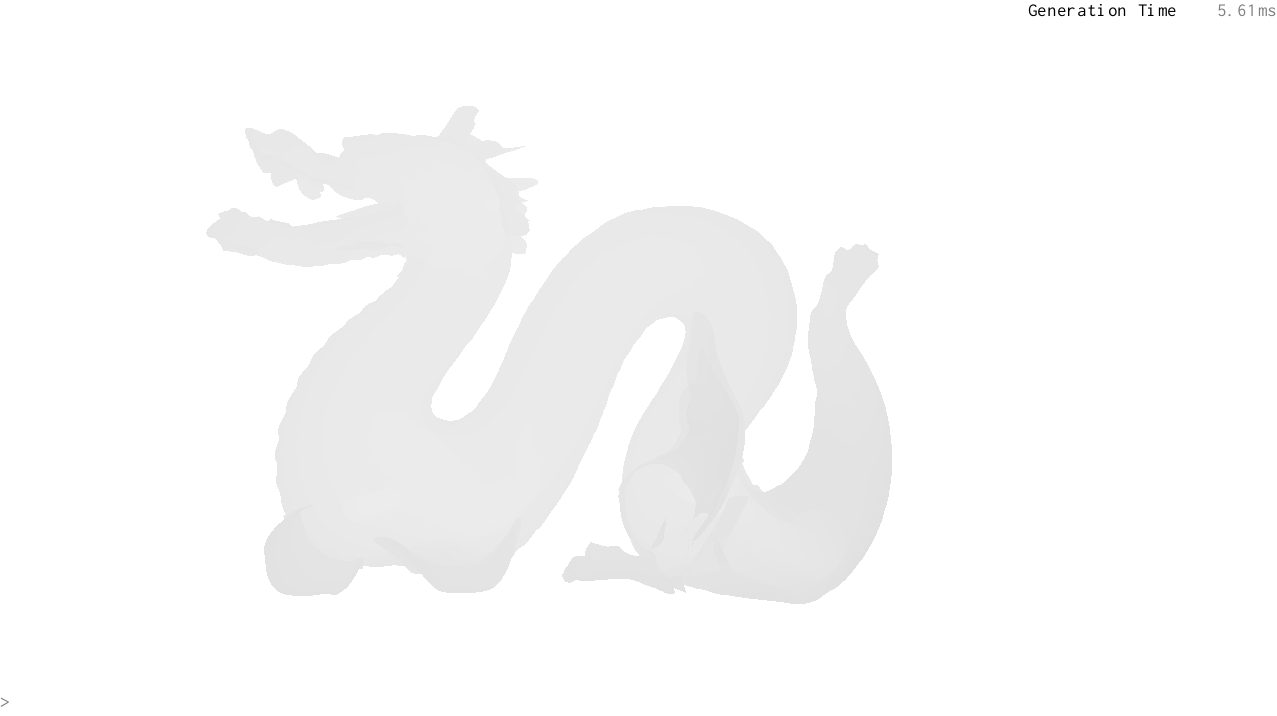
\includegraphics[scale=0.1,trim=0 0 0 -5]{img/results/g-buffer/depths-2layer-2} \\
\hline
\emph{Normals} &
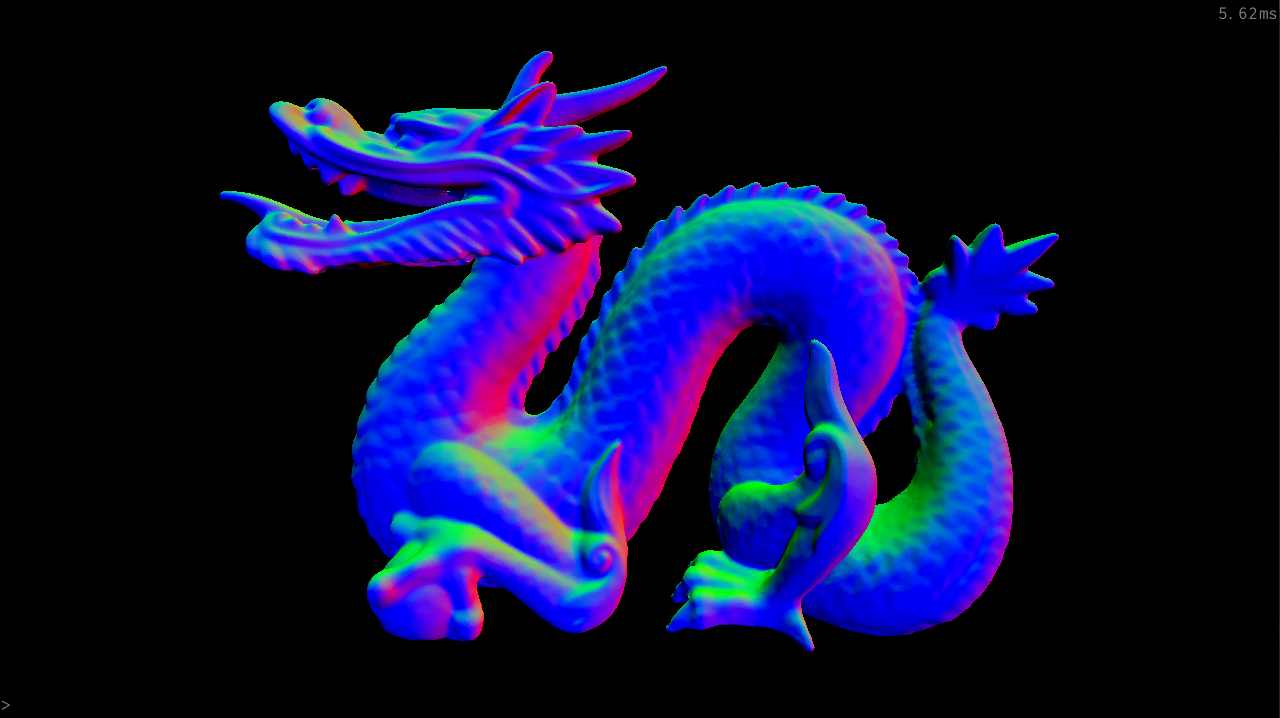
\includegraphics[scale=0.1,trim=0 0 0 -5]{img/results/g-buffer/normals-2layer-1} &
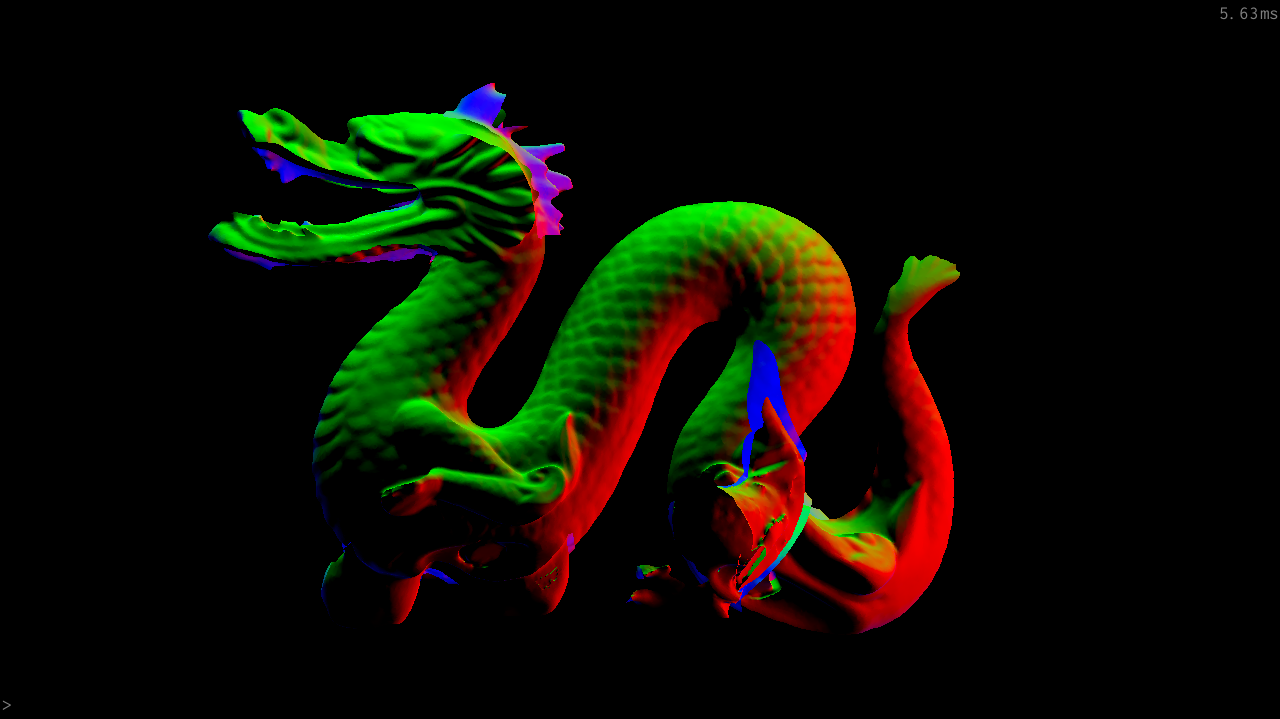
\includegraphics[scale=0.1,trim=0 0 0 -5]{img/results/g-buffer/normals-2layer-2} \\
\hline
\end{tabular}
\caption{Table with resulting Normal and Depth textures from the G-buffer generation.}
\label{table-buffers}
\end{table}

I also did a number of tests on the running time. One in which I rasterise two layers of geometry with the single-pass pipeline, and one in which only one layer is rasterised. I include a control result from the \emph{conference} scene for comparison to the double-layered result. These results can be seen in table \ref{table-gbuffer-time}.

\begin{table}[!ht]
\centering
\begin{tabular}{| c | p{2.5cm} | p{2.5cm} | p{2.5cm} |}
\hline
 & \emph{Dragon} 1 layer & \emph{Dragon} 2 layers & \emph{Conference} 2 layers\newline (Control) \\
\hline
\emph{Average Time} & 2.95ms & 5.62ms & 2.57ms \\
\hline
\end{tabular}
\caption{Table of G-buffer generation times.}
\label{table-gbuffer-time}
\end{table}

\subsection{Discussion}
For table \ref{table-buffers}, the resulting buffers are in line with what we would expect from the G-buffer generation. While it is hard to verify the depth-texture correctness, since it is stored in an exponential format and this appears mostly the same colour, we can tell by the results of the lambertian shader that the positions are, indeed correct. We can tell that the normals are correctly stored based on the colours shown. Since they are stored in view-space, we would expect front-facing fragments to appear blue as view-space coordinates have the camera oriented along negative Z. We'd expect increasingly red values for right-facing fragments and increasingly green values for upwards-facing fragments, which is exactly what we have.

The interesting thing about this test is the results shown in \ref{table-gbuffer-time}. For our single-pass generation pipeline, in which we transform geometry once in the vertex shader, we'd expect somewhat higher generation time for rasterising to two layers, but not almost doubled values. What this means is that the majority of time spent in rasterisation is spent on interpolation of vertices and normals rather than the transformations themselves. That said, the single-pass method is still superior to a potential double-pass one, since the double pass one would have to use two textures, which would be slower to read values from and would make for more messy code.

\section{Lambertian and Shadow Mapping}

\begin{table}[!ht]
\begin{center}
\begin{tabular}{| c | p{2.5cm} | p{2.5cm} | p{2.5cm} | p{2.5cm} |}
\hline
Model & \emph{Dragon} & \emph{Dragon} & \emph{Dragon} & \emph{Conference} \\
\hline
Rendering &
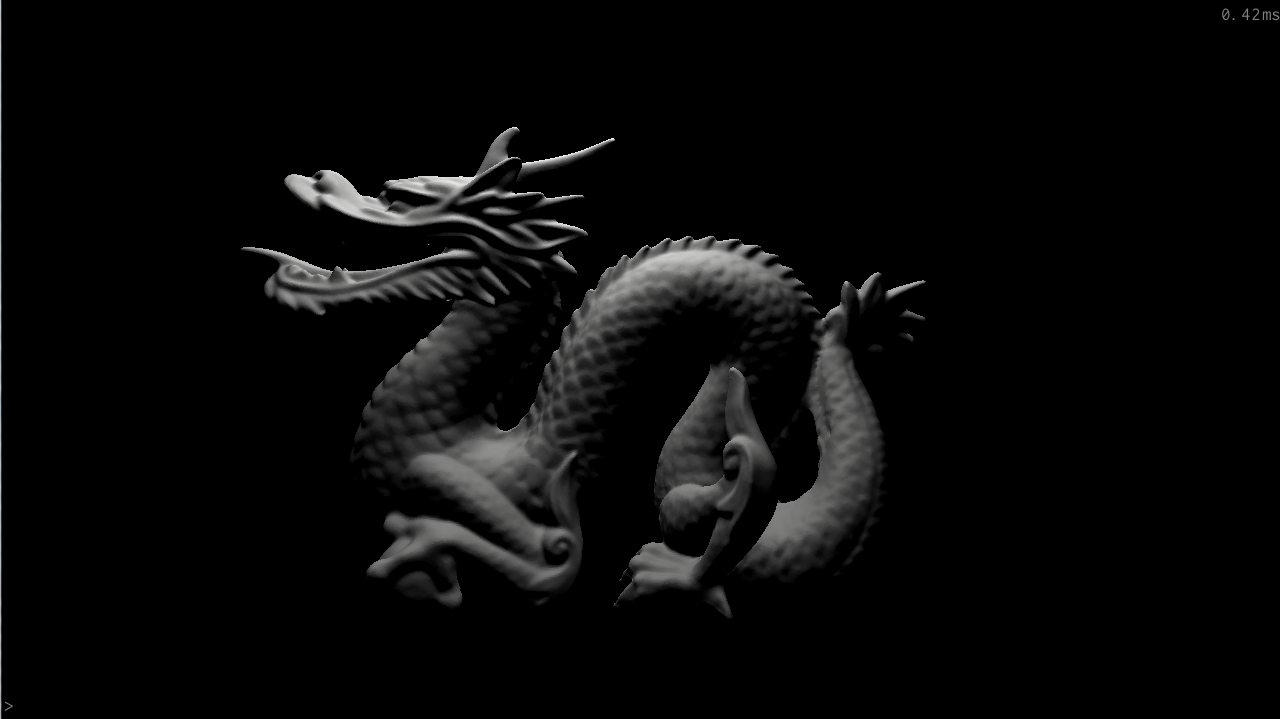
\includegraphics[scale=0.08,trim=0 0 0 -5]{img/results/lambertian/noocclusion-dragon} &
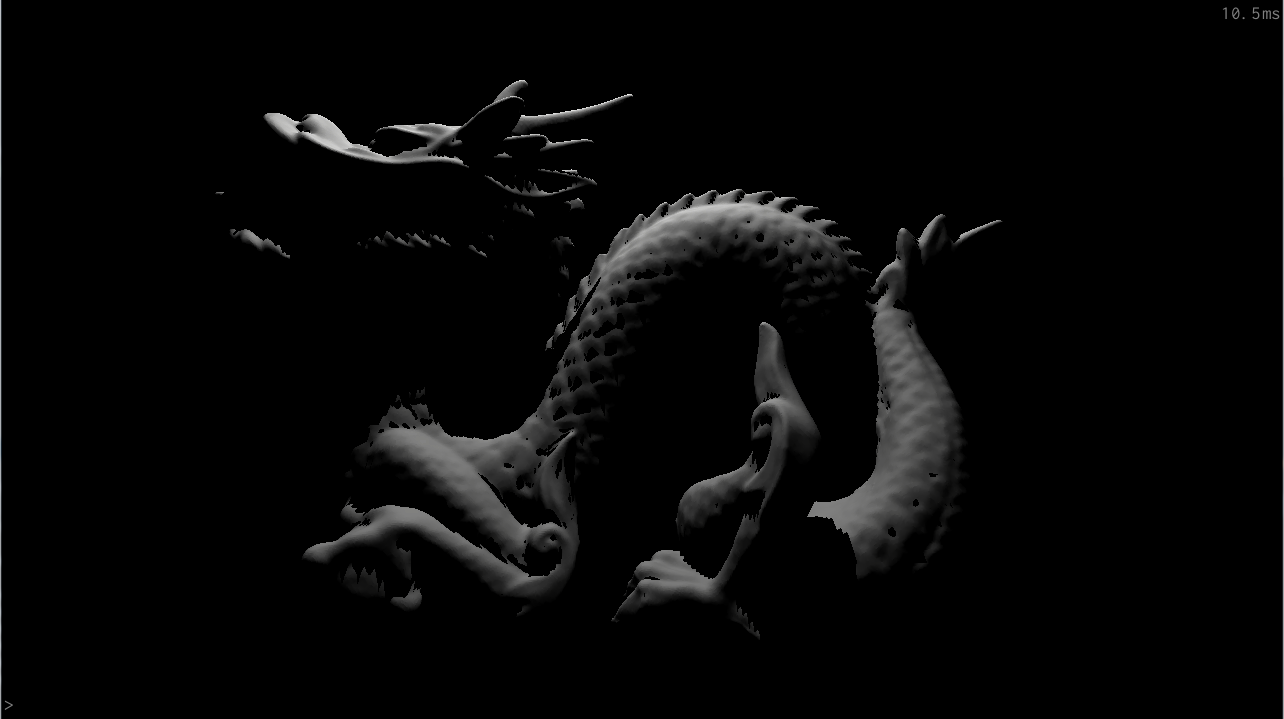
\includegraphics[scale=0.08,trim=0 0 0 -5]{img/results/shadowmap/480by480} &
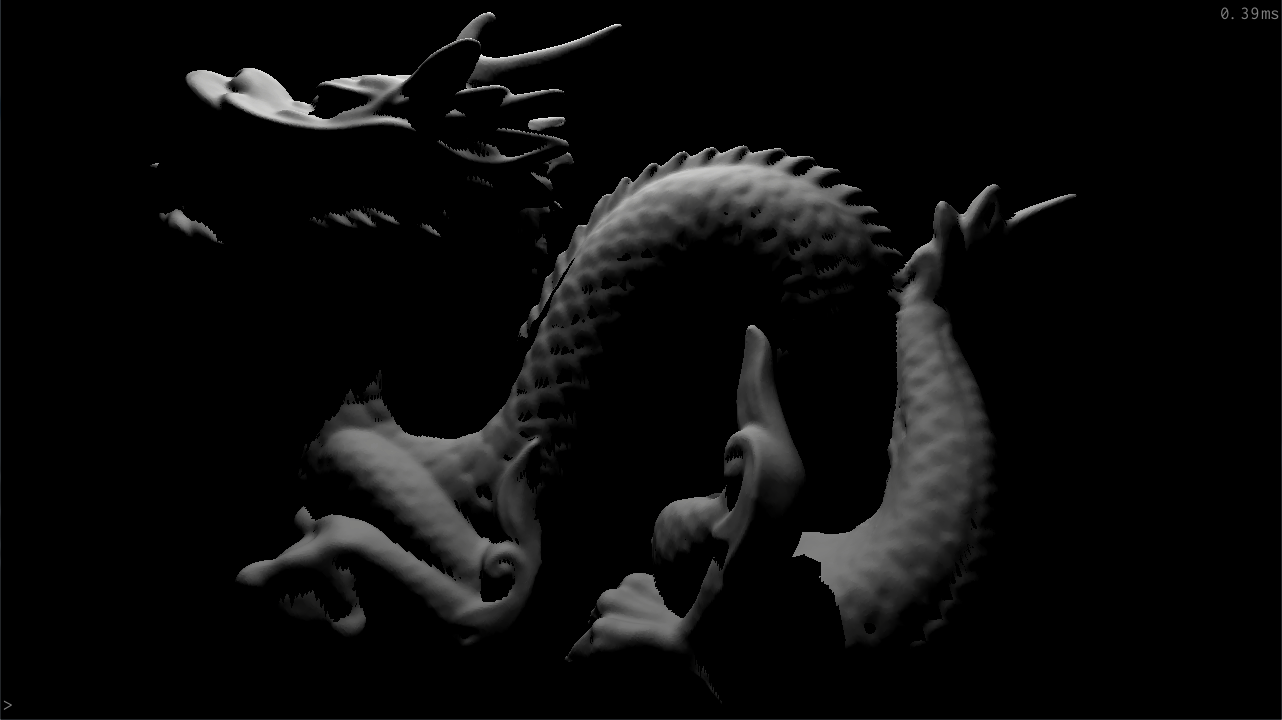
\includegraphics[scale=0.08,trim=0 0 0 -5]{img/results/lambertian/occlusion-dragon} &
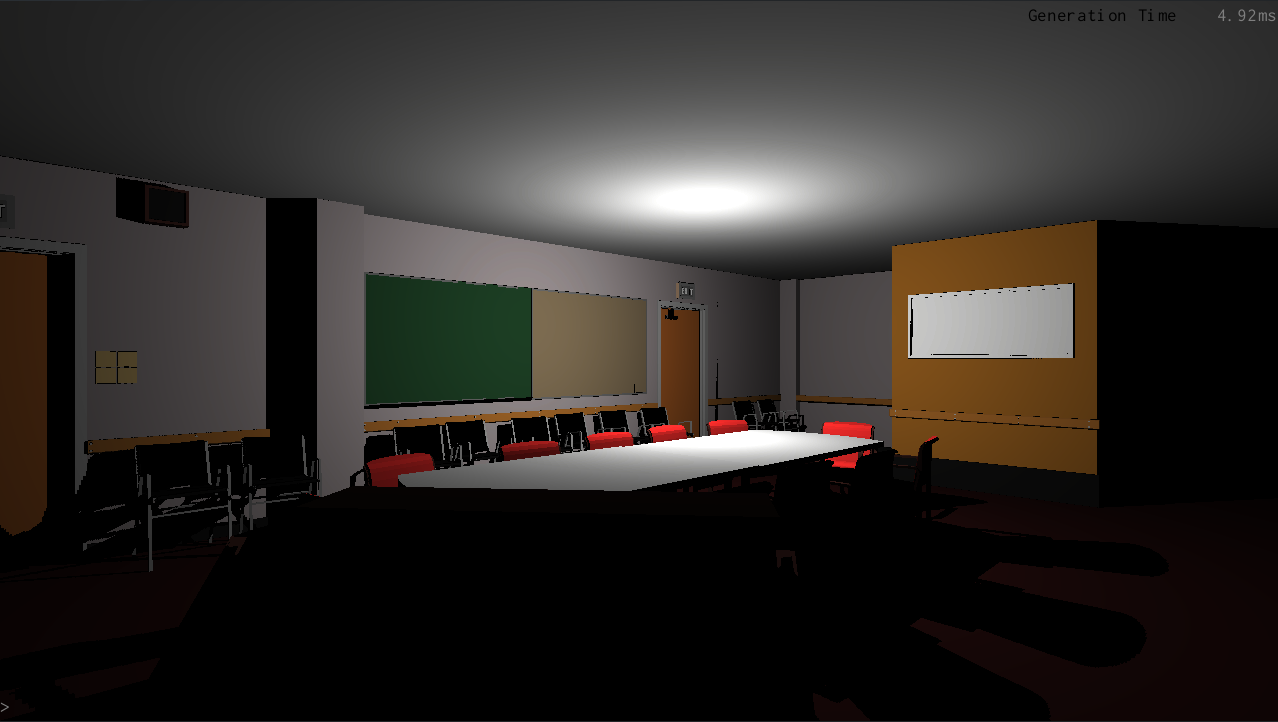
\includegraphics[scale=0.08,trim=0 0 0 -5]{img/results/shadowmap/conference1024x1024} \\
\hline 
\emph{Map Size} & No occlusion & 480 & 1024 & 1024\\
\hline
\emph{Lambertian Time} & 0.36ms & 0.36ms & 0.36ms & 0.36ms\\
\hline
\emph{Shadowmap Time} & 0.0ms & 10.4ms & 10.6ms & 4.90ms\\
\hline
\end{tabular}
\caption{Tests done on lambertian shading and shadow map generation. Shadowmap Time denotes the time spent to generate the shadow map.}
\label{table-lambert}
\end{center}
\end{table}

\subsection{Discussion}
A single run of the lambertian filter takes 0.36ms regardless of scene complexity and use of a shadow map. The independence from scene complexity is expected, since it is the primary feature of deferred rendering; however, the result being independent of use of a shadow map is unexpected. It is possible that the driver "guessed" that shadow mapping is going on and has done some optimisations to the shader behind the scenes. Alternatively my timer has somehow produced the wrong result. Whether or not to do scene reconstruction is a question of trading VRAM usage for performance. That said, 0.36ms to draw an occluded light source is a very reasonable result, considering we're doing per-fragment transformations and saving 64 bits of buffer space per fragment.

 I included the dragon model in the table because it demonstrates omni-directional shadow maps well. You can see that all objects in the scene are considered in the occlusion test, demonstrating that the shadow map works in all directions. As expected, the quality of the shadow increases between the 480x480 resolution per face to the 1024x1024 resolution per face, and luckily it has very little impact on performance. However, maintaining six 1024x1024 32-bit textures to test occlusion for a single light source is a big memory concern. The shadow map drawing time appears to be linearly dependent upon geometric complexity, which is also expected since we rasterise the scene to generate it. Spending 10ms on a single shadow map is infeasible for real-time applications if you wish to have time for other effects, and as such I would probably not recommend using this method unaltered. A possible alternative would be dual paraboloid shadow-maps which require only two textures, and thus only the geometry rasterised twice and has a third of the memory footprint. As a proof of concept, however, the cube shadowmap works as intended.

One final note is that there are some shadow artefacts (acne) on the dragon, and if you look closely at the corners of the conference room. It could be alleviated by adding more bias to the comparison, but adding any more bias causes peter panning in both the conference room and cornell box scenes. The current bias of $0.0001f$ was the best compromise between the two.

\section{Radiosity}
I use a sample radius of 300 to ensure that as large a part of screen-space as possible is covered, without losing too many samples by sampling outside of it. I also ensure that any value further away than 500 units is not considered part of the hemisphere, to maintain some enforcement of world-space consistency. Figure \ref{table-rad-samples} shows the consequence of changing the number of spiral taps done in the shader, while table \ref{table-rad-bounces} demonstrates the consequences of different different numbers of bounces. \ref{fig-rad-comparison} is the control in this case.

\begin{table}[!ht]
\begin{center}
\begin{tabular}{| c | p{3.5cm} | p{3.5cm} | p{3.5cm} |}
\hline
&
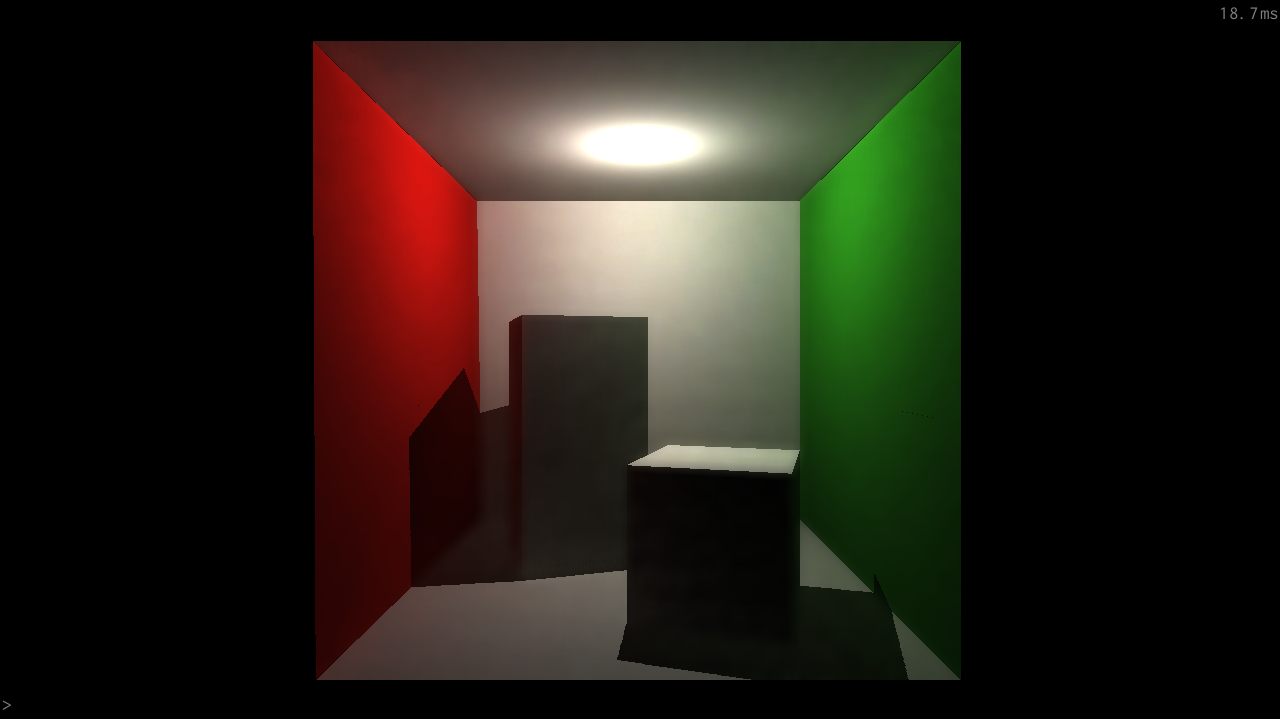
\includegraphics[scale=0.1,trim=0 0 0 -5]{img/results/radiosity/11samples} &
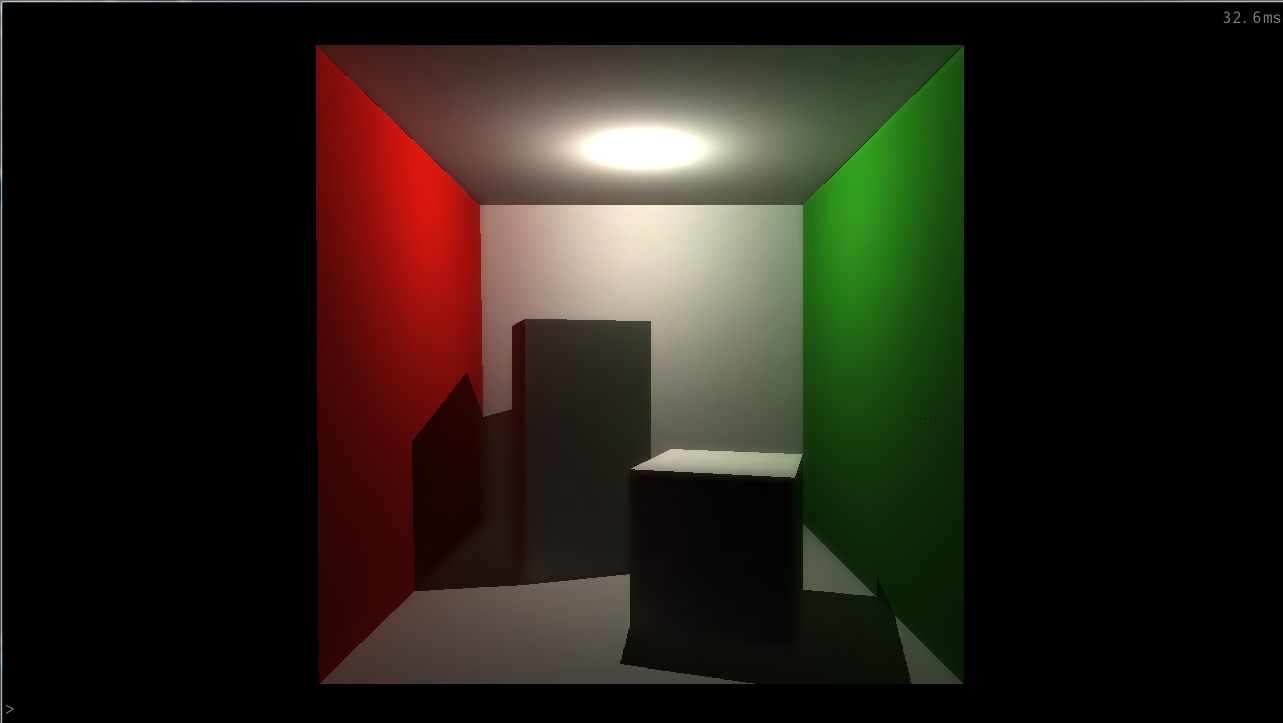
\includegraphics[scale=0.1,trim=0 0 0 -5]{img/results/radiosity/23samples} &
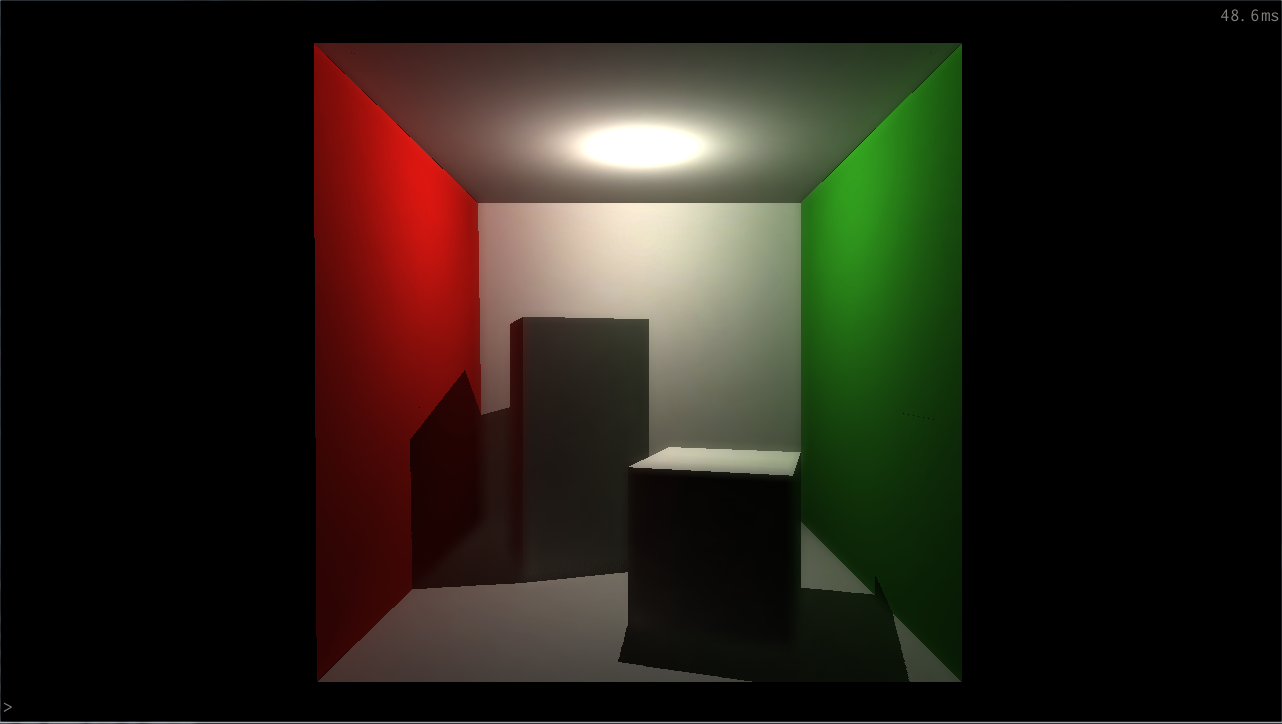
\includegraphics[scale=0.1,trim=0 0 0 -5]{img/results/radiosity/37samples} \\
\hline
\emph{Samples} & 11 & 23 & 37 \\
\hline
\emph{Frame Time} & 18.7ms & 32.6ms & 48.6ms\\
\hline
\end{tabular}
\caption{Table of frame times based on sample taps used to approximate radiosity. Time is for 2 bounces of radiosity.}
\label{table-rad-samples}
\end{center}
\end{table}

\begin{table}[!ht]
\begin{center}
\begin{tabular}{| c | p{3.5cm} | p{3.5cm} | p{3.5cm} |}
\hline
&
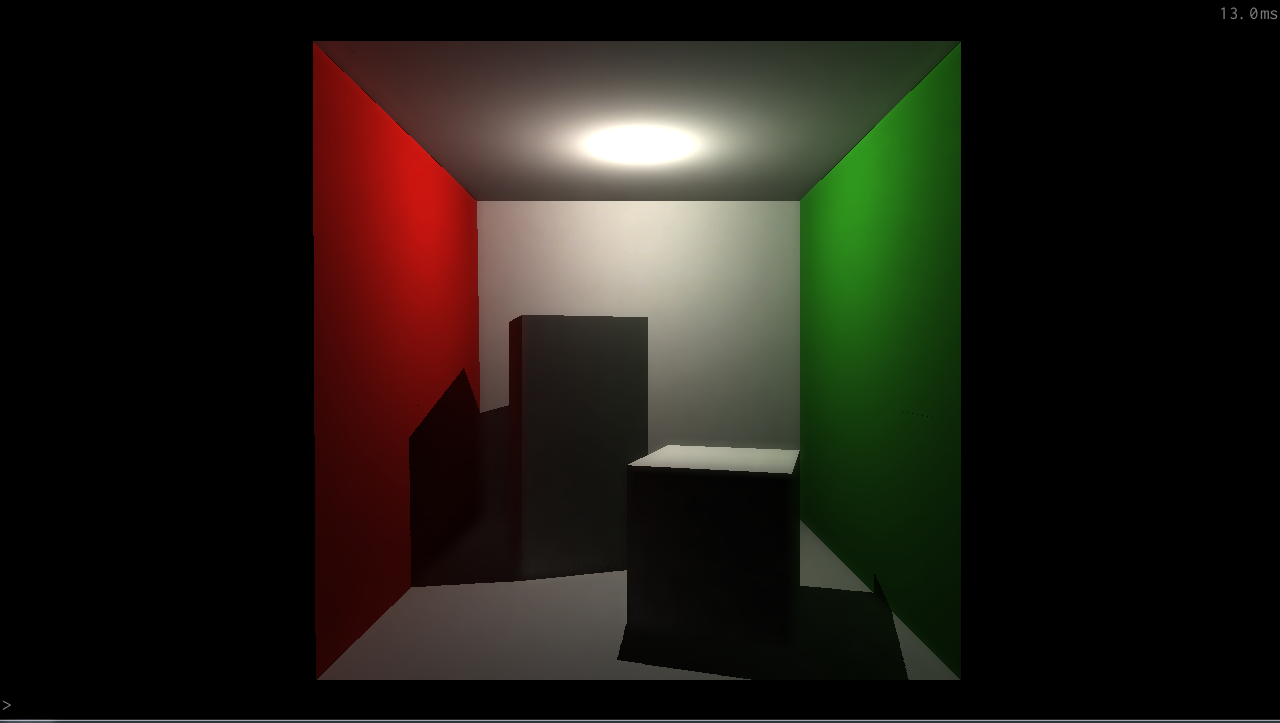
\includegraphics[scale=0.1,trim=0 0 0 -5]{img/results/radiosity/1bounce} &
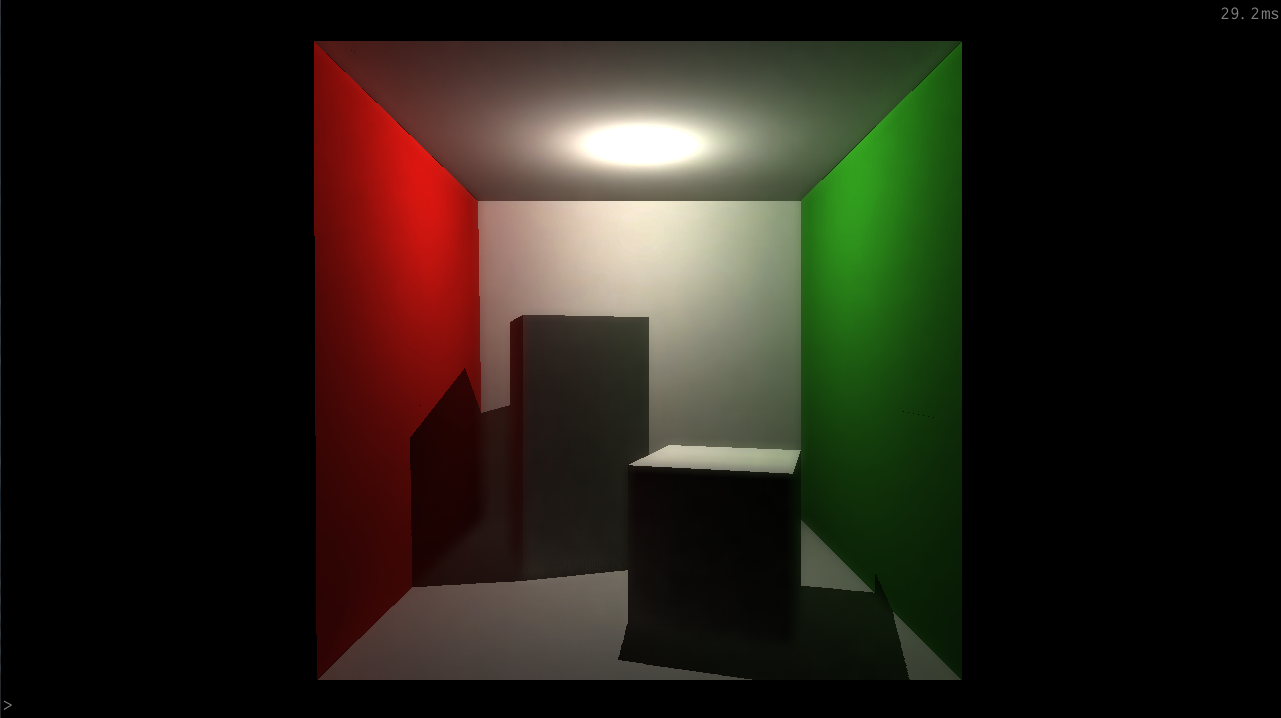
\includegraphics[scale=0.1,trim=0 0 0 -5]{img/results/radiosity/2bounce} &
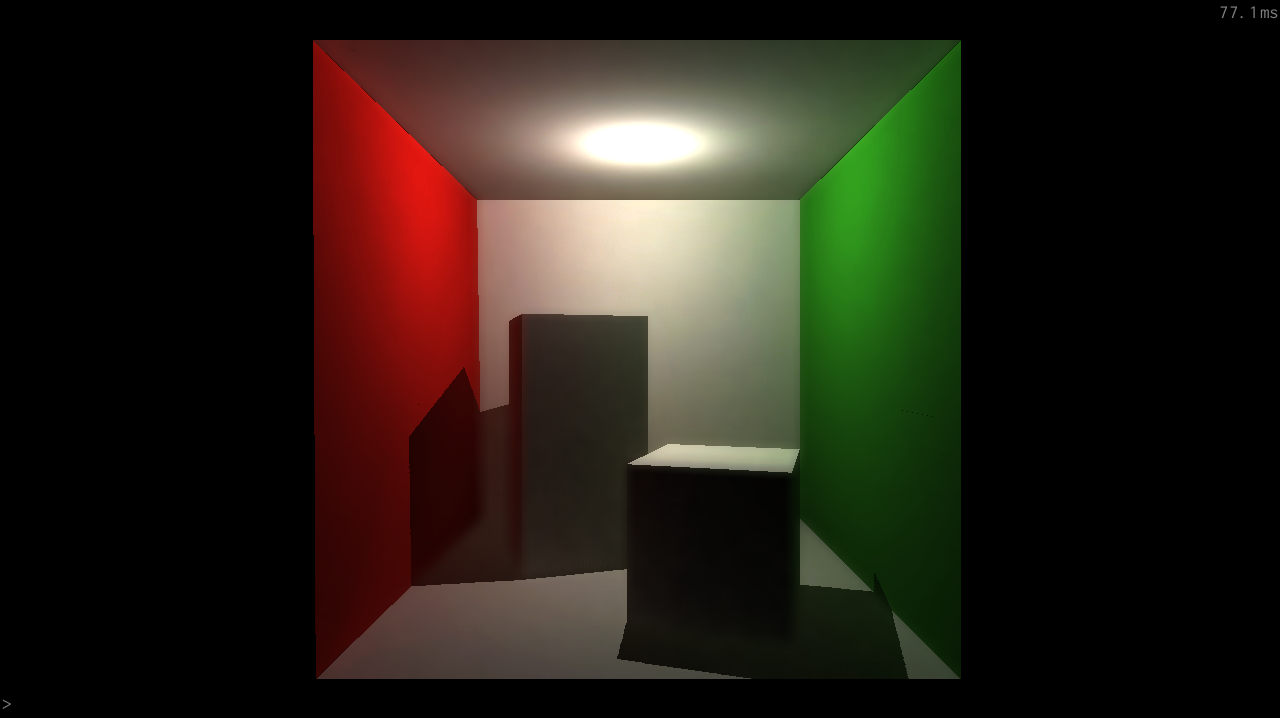
\includegraphics[scale=0.1,trim=0 0 0 -5]{img/results/radiosity/5bounce} \\
\hline
\emph{Bounces} & 1 & 2 & 5 \\
\hline
\emph{Frame Time} & 13.0ms & 29.1ms & 77.1ms\\
\hline
\end{tabular}
\caption{Table for the number of radiosity bounces used. Sample taps is 20.}
\label{table-rad-bounces}
\end{center}
\end{table}

\begin{figure}[!ht]
\centering
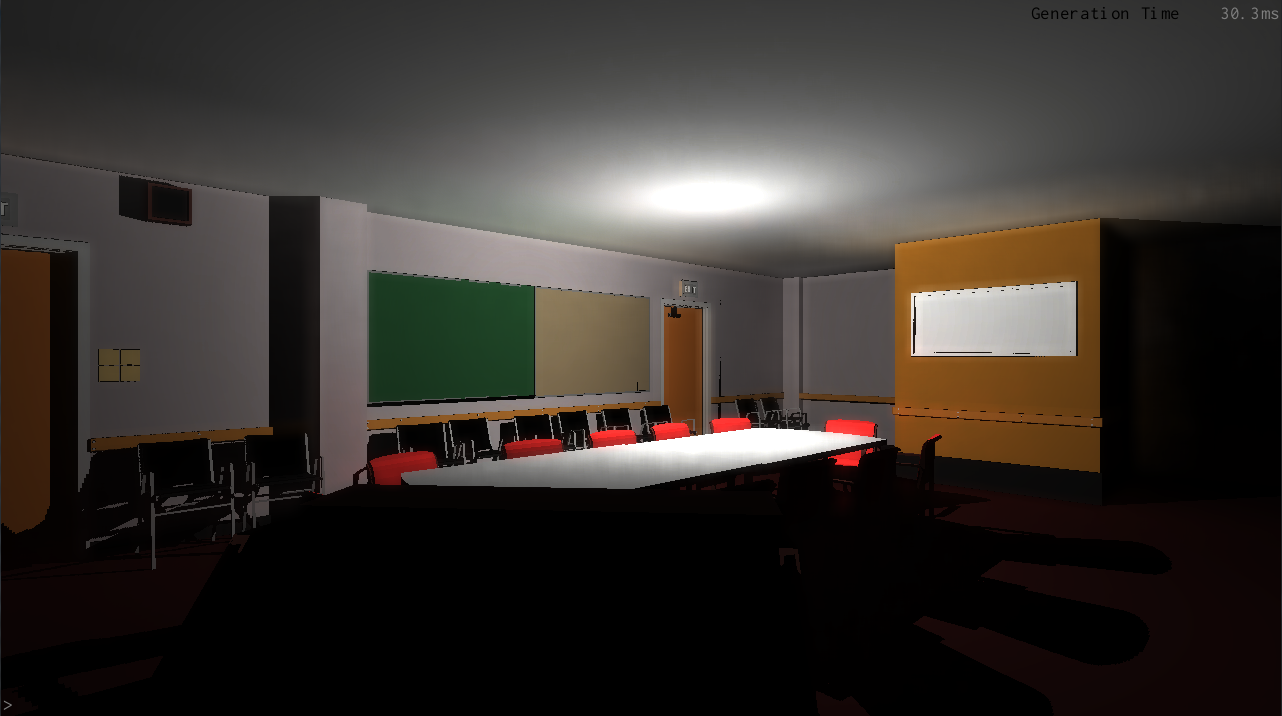
\includegraphics[scale=0.3]{img/results/radiosity/comparison}
\caption{Radiosity control scene (\emph{Conference}). 2 bounces, 23 samples. Time: 32.5ms}
\label{fig-rad-comparison}
\end{figure}

\subsection{Discussion}
Radiosity results look like expected, considering I'm not doing any occlusion testing. The red and green walls are bleeding unto the boxes, ceiling and floor, and the part of the room occluded by the large box is lit up. Rendering time rises linearly with the number of samples (seems to be around 1ms per sample.) As expected the result becomes smoother as the number of samples increases. For 11 samples, there's a lot of risidual noise from the randomisation, while it is mostly unnoticeable for 23 samples, and appears almost completely smooth for 37 samples. I would consider 23 samples an acceptable result, but 32.6ms is a \emph{lot} of time to spend on a single filter. However, this can be alleviated by implementing temporal filtering in which subsequent bounces are done in subsequent frames, and the result is filtered to account for the changing energy levels. Even with a single bounce of radiosity, though, the total time is 13ms or so, which is still a lot of time to be spending on a single effect.

For the number of bounces the time also seems to rise linearly with the number of bounces. It is a bit weird that the time more than doubles between bounce 1 and 2, but I consider that a measurement error of some nature. You can see the light propagating progressively from 1 to 5 bounces; for instance, the green and red contributions on the ceiling become increasingly noticeable, and the occluded spot behind the tall box becomes more and more illuminated. Radiosity seems to stop propagating after 4-5 bounces, which makes sense. Energy is lost with every bounce, and the textures used only allow for a certain amount of precision, meaning additions to the cumulating texture (containing all bounces and lambertian) become insignificant after a while.

\section{SSAO}

\begin{table}[!ht]
\begin{center}
\begin{tabular}{| c | p{3.5cm} | p{3.5cm} | p{3.5cm} |}
\hline
&
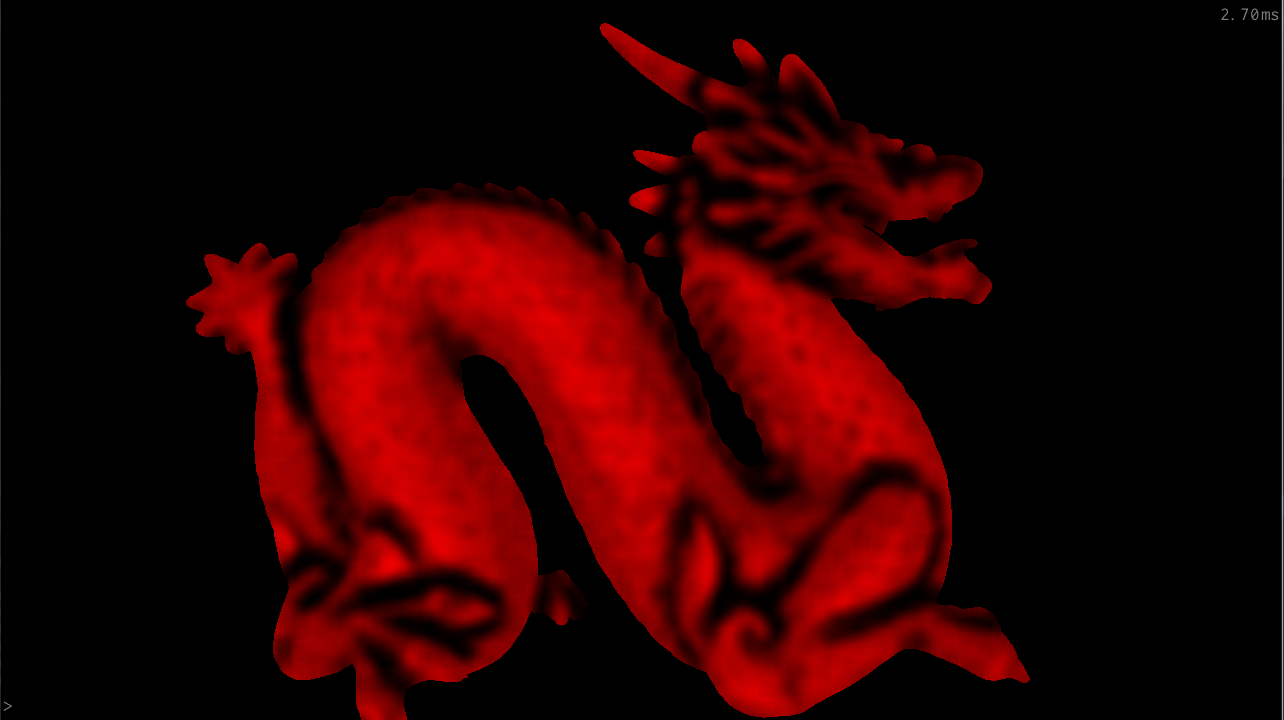
\includegraphics[scale=0.1,trim=0 0 0 -5]{img/results/ssao/11samplesdragon} &
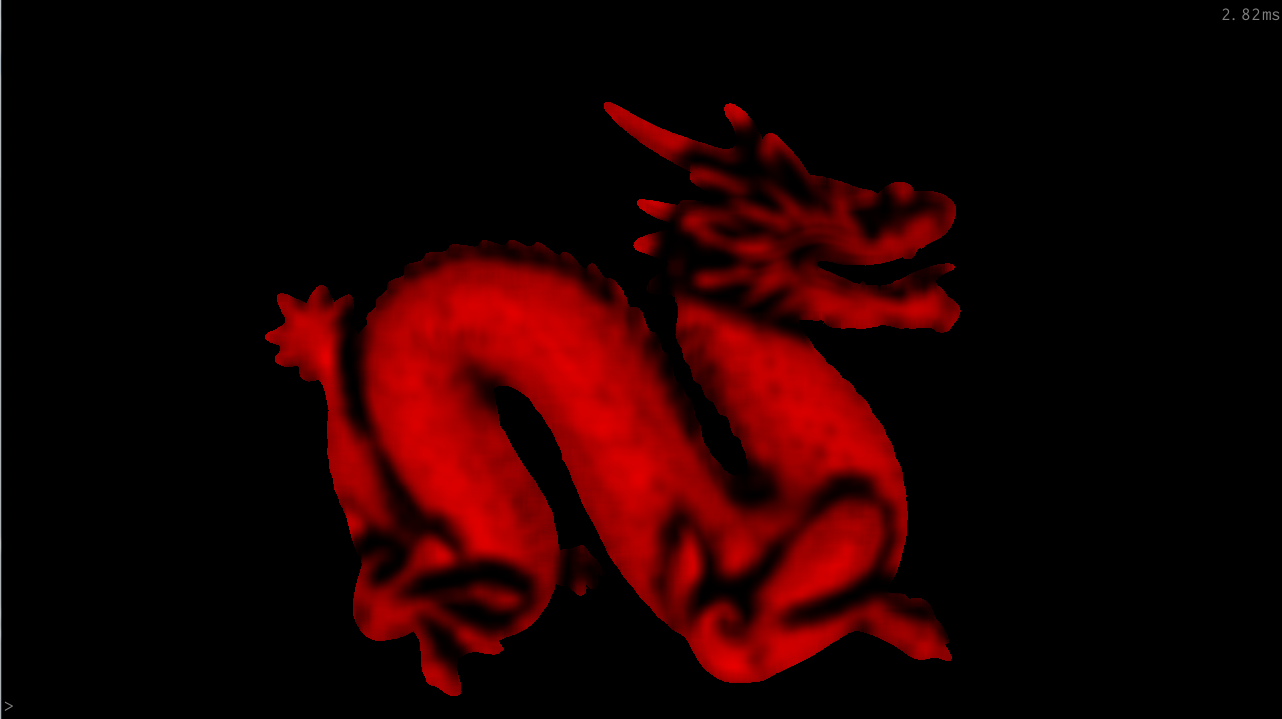
\includegraphics[scale=0.1,trim=0 0 0 -5]{img/results/ssao/23samplesdragon} &
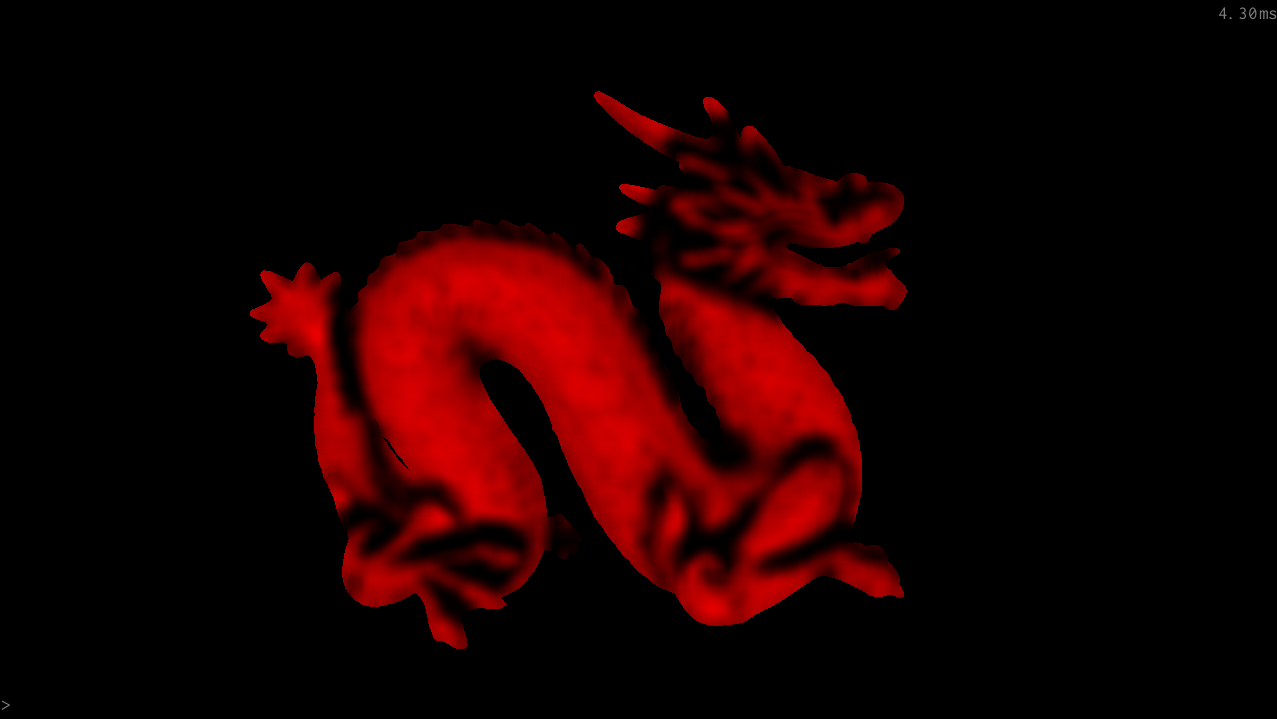
\includegraphics[scale=0.1,trim=0 0 0 -5]{img/results/ssao/37samplesdragon} \\
\hline
\emph{Samples} & 11 & 23 & 37 \\
\hline
\emph{Frame Time} & 2.71ms & 2.80ms & 3.17ms\\
\hline
\end{tabular}
\caption{Time to draw SSAO based on number of samples.}
\label{table-ssao-samples}
\end{center}
\end{table}

\subsection{Discussion}
The first thing I noticed is that there's very little difference in quality between the three sampling amounts, but I would consider them all acceptable. However, what's interesting to note is that there's very little difference in filtering time across the three levels. Additionally, the time taken is significantly lower than that of radiosity. There could be a number of reasons for this; either the texture is stored in such a way that adjacent values are faster to read than values that are far from each other. Since SSAO uses a scree-space sampling radius of around 30 and radiosity's is 300, if this were the case, it would explain the big difference. The other is that the \verb=R11F_G11F_B10F= textures used for radiosity, and the fact that radiosity has blending as well, creates so much overhead that the shader runs much slower than it could've if the texture formats were more appropriate. Using more textures to generate the radiosity result probably also contributes to this. This is in accordance with the finding that changing the normal texture to \verb=GL_RGB16F= actually improved performance on all filters by quite a bit.

Since SSAO is a one-time filter per frame, 2-3ms isn't too bad considering the results it produces.

\section{Gaussian Filter}

\begin{table}[!ht]
\begin{center}
\begin{tabular}{| c | p{5cm} | p{5cm} |}
\hline
&
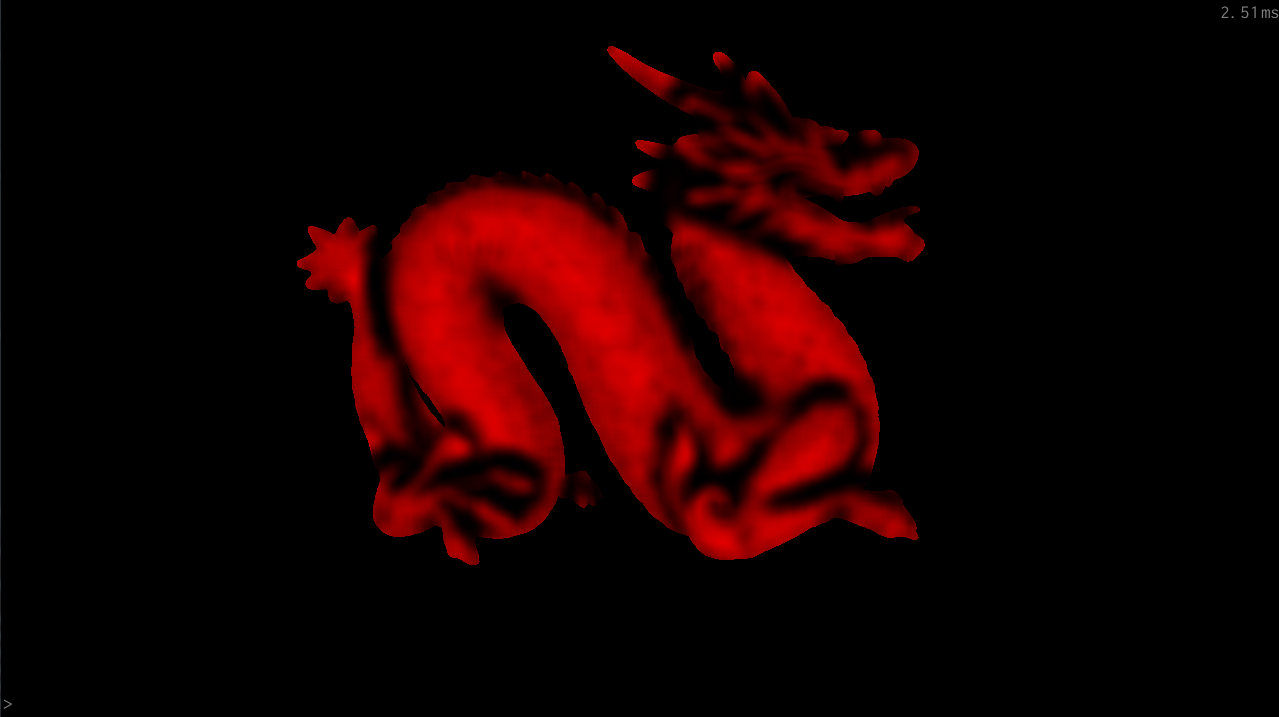
\includegraphics[scale=0.15,trim=0 0 0 -5]{img//results/ssao/dragon-gauss} &
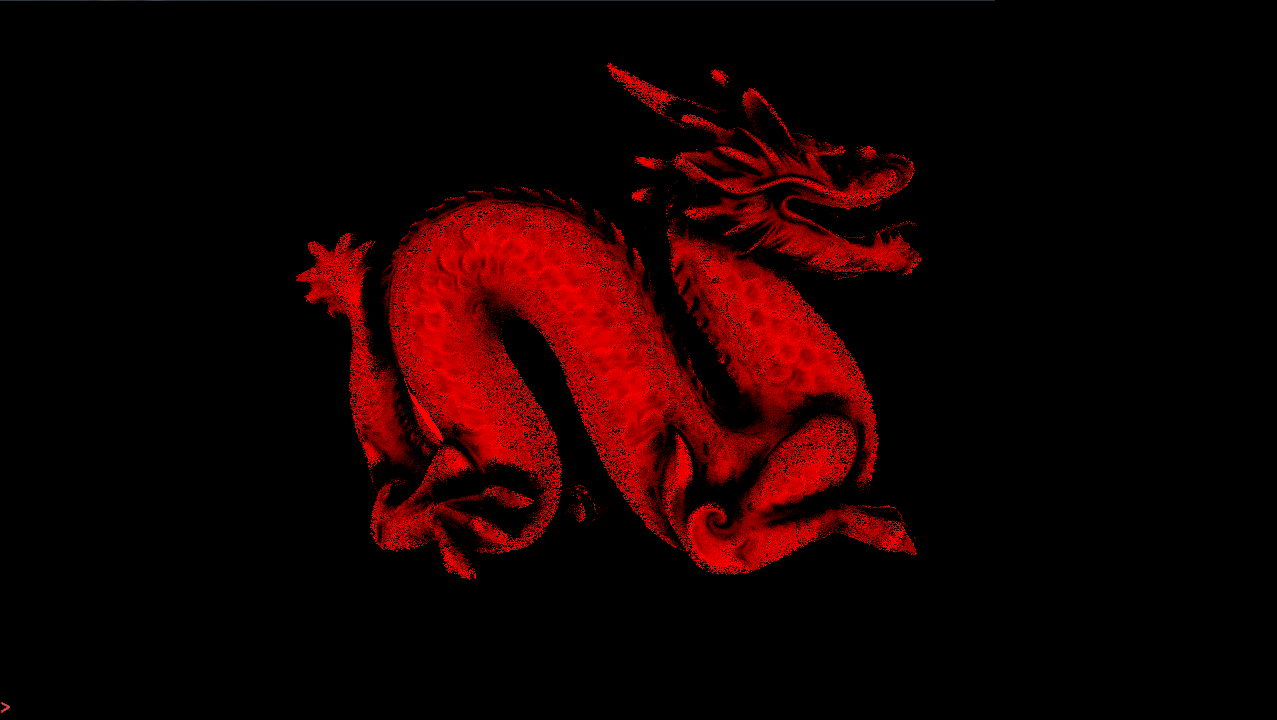
\includegraphics[scale=0.15,trim=0 0 0 -5]{img/results/ssao/dragon-nogauss} \\
\hline
\emph{Filtered} & Yes & No \\
\hline
\emph{Frame Time} & 2.50ms & 1.61ms \\
\hline
\end{tabular}
\caption{Gussian filtering on SSAO. Radius = 20}
\label{table-gauss-ssao}
\end{center}
\end{table}

\begin{table}[!ht]
\begin{center}
\begin{tabular}{| c | p{5cm} | p{5cm} |}
\hline
&
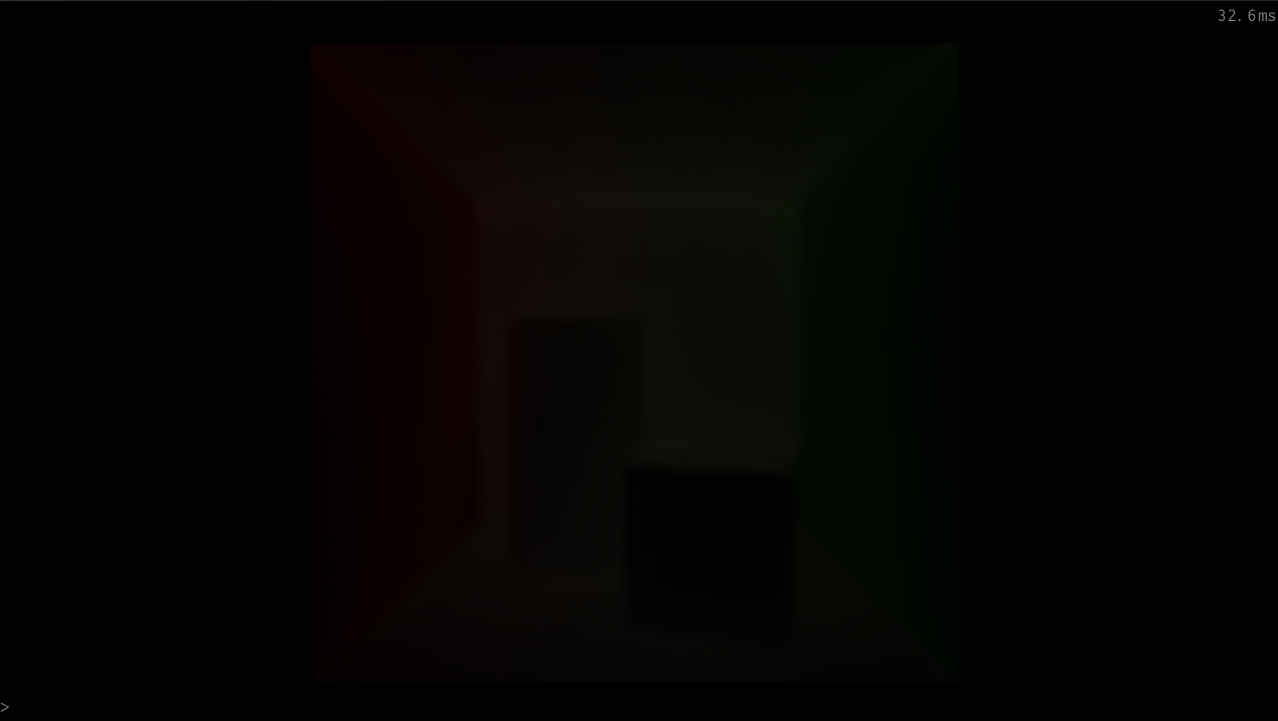
\includegraphics[scale=0.15,trim=0 0 0 -5]{img//results/radiosity/wBlend} &
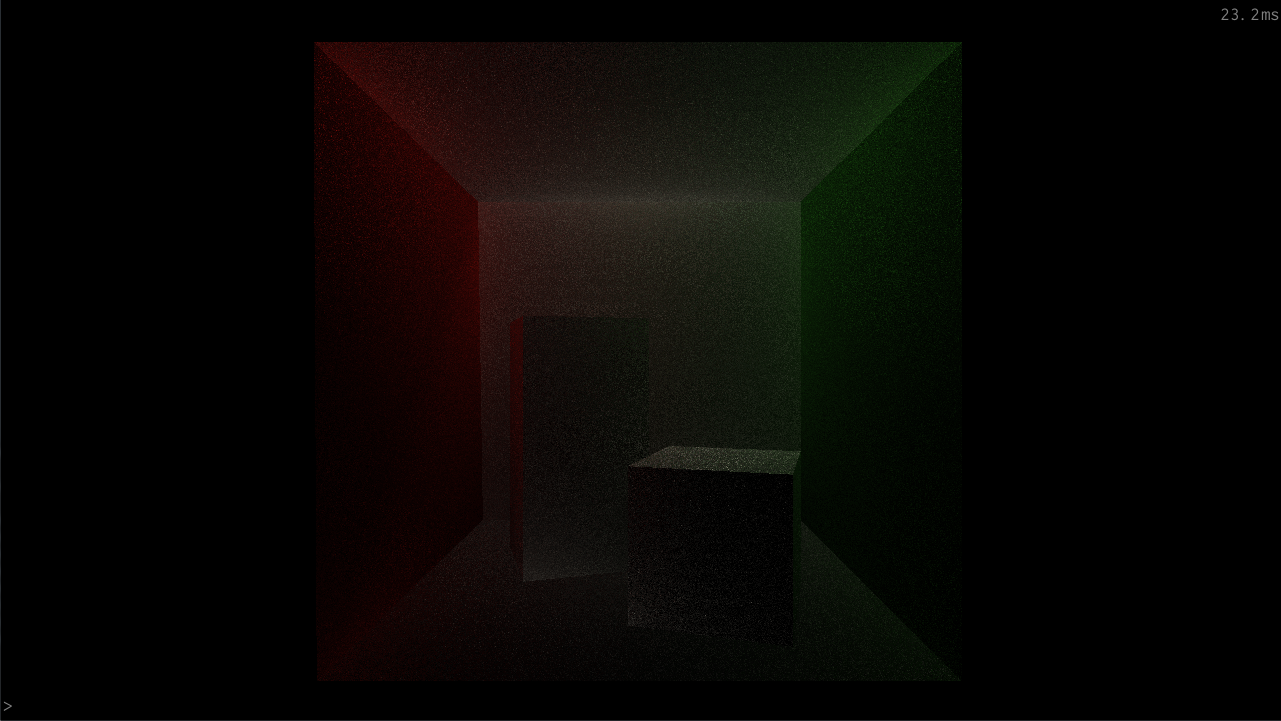
\includegraphics[scale=0.15,trim=0 0 0 -5]{img/results/radiosity/woBlend} \\
\hline
\emph{Filtered} & Yes & No \\
\hline
\emph{Frame Time} & 32.6ms & 23.2ms \\
\hline
\end{tabular}
\caption{Gussian filtering on Radiosity bounce. Gauss radius = 20, 2 bounces, 23 samples.}
\label{table-gauss-rad}
\end{center}
\end{table}

\subsection{Discussion}
The benefit of applying the modified Gaussian filter is immediately visible for both radiosity and SSAO. For a high enough radius (I found 20 to be the best balance,) the random noise is almost completely unnoticeable. You can tell on the right hand side that there are a lot of black spots on the SSAO result, and high variance on the radiosity result, which are both entirely gone after the filter has been applied. One weird thing, though, is the fact that filtering the SSAO only adds .89ms to the time, whereas filtering the radiosity adds around 4ms per frame. This is the primary reason I think the high rendering times on the radiosity filter is caused by one of the choices I made in regards to texture formats and blending, since the Gaussian filters for the two are identical except for those two facts.

Another thing to note is that while the depth-based edge-aware filter does alleviate some bleeding between surfaces that are at different depths, surfaces with different normals still bleed into each other, creating blurry results around edges of the same object. A way to alleviate this in an efficient manner would be to run an edge-detection filter that could be used by all Gaussian filters. It would hold a single float of value 0 or 1, which would be determined by some factor of depth and the normal's relation to surrounding normals. When the Gaussian filter hits whatever value we say is the edge value (probably a 1 for positive,) it would stop taking contributions in that direction. It does mean we would have to loop through the source texture from the center, in stead of from -radius to radius, but that is a minor fix.

As it is, considering the efficiency of the filter in smoothing out results, I'd consider 0.9ms a reasonable time for the result it gives.

\section{Composite Rendering}
The following table contains composite renderings of all three scenes with one layer and two layers. The composite is the sum of radiosity, and SSAO multiplied by ambient reflectance.

\begin{table}[!ht]
\begin{center}
\begin{tabular}{| c | p{3.5cm} | p{3.5cm} | p{3.5cm} |}
\hline
\emph{Model} & \emph{Dragon} & \emph{Cornell} & \emph{Conference} \\
\hline
\multicolumn{4}{|c|}{\emph{One Layer}} \\
\hline
\emph{Rendering} &
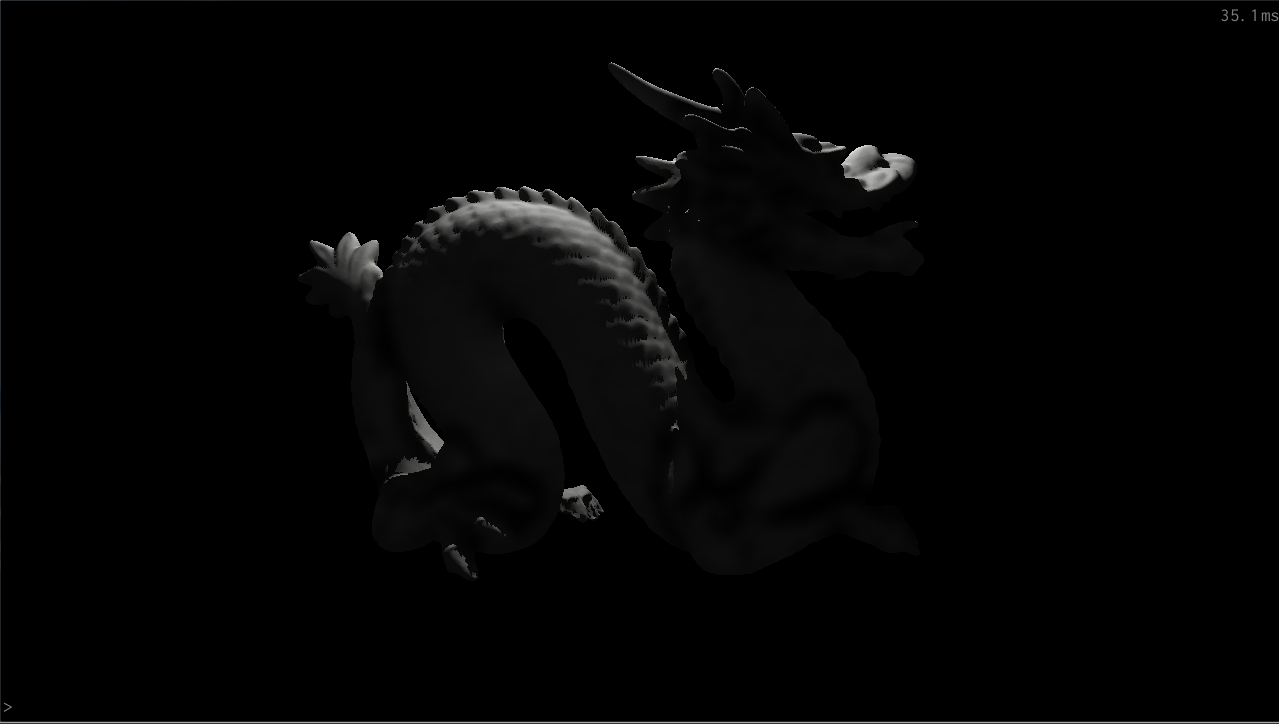
\includegraphics[scale=0.1,trim=0 0 0 -5]{img/results/composite/dragon-1layer} &
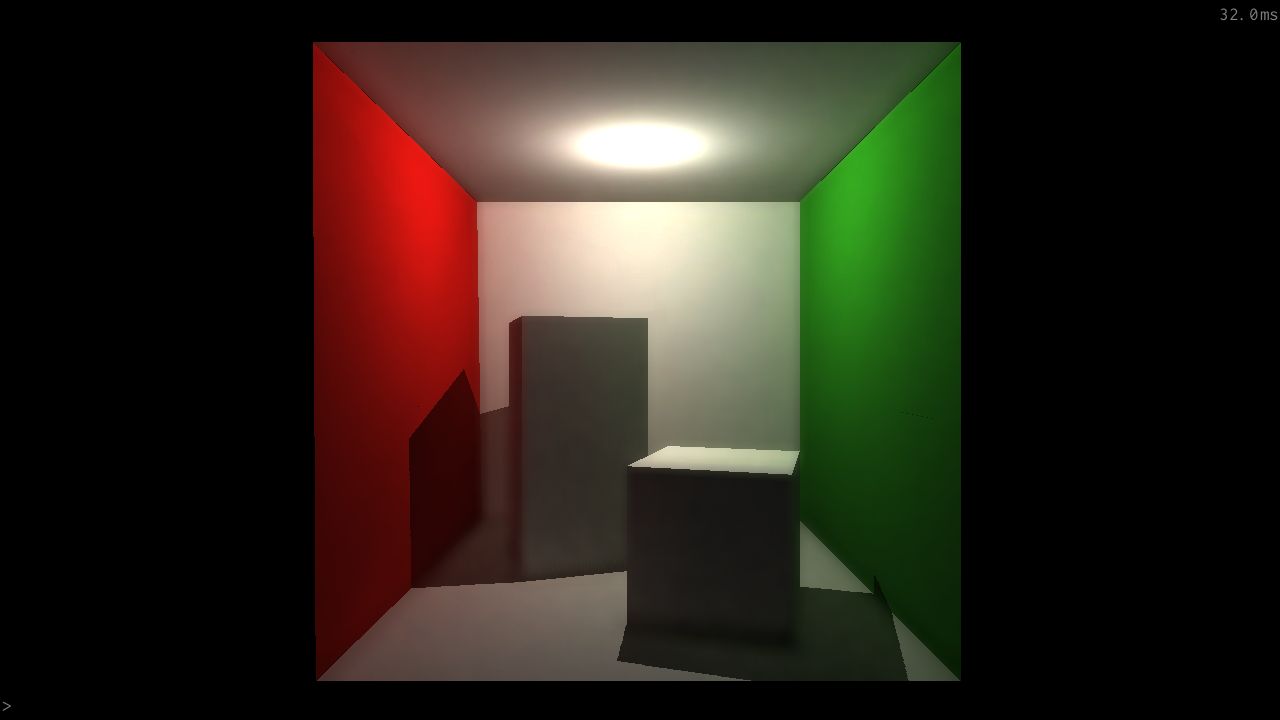
\includegraphics[scale=0.1,trim=0 0 0 -5]{img/results/composite/cornell-1layer} &
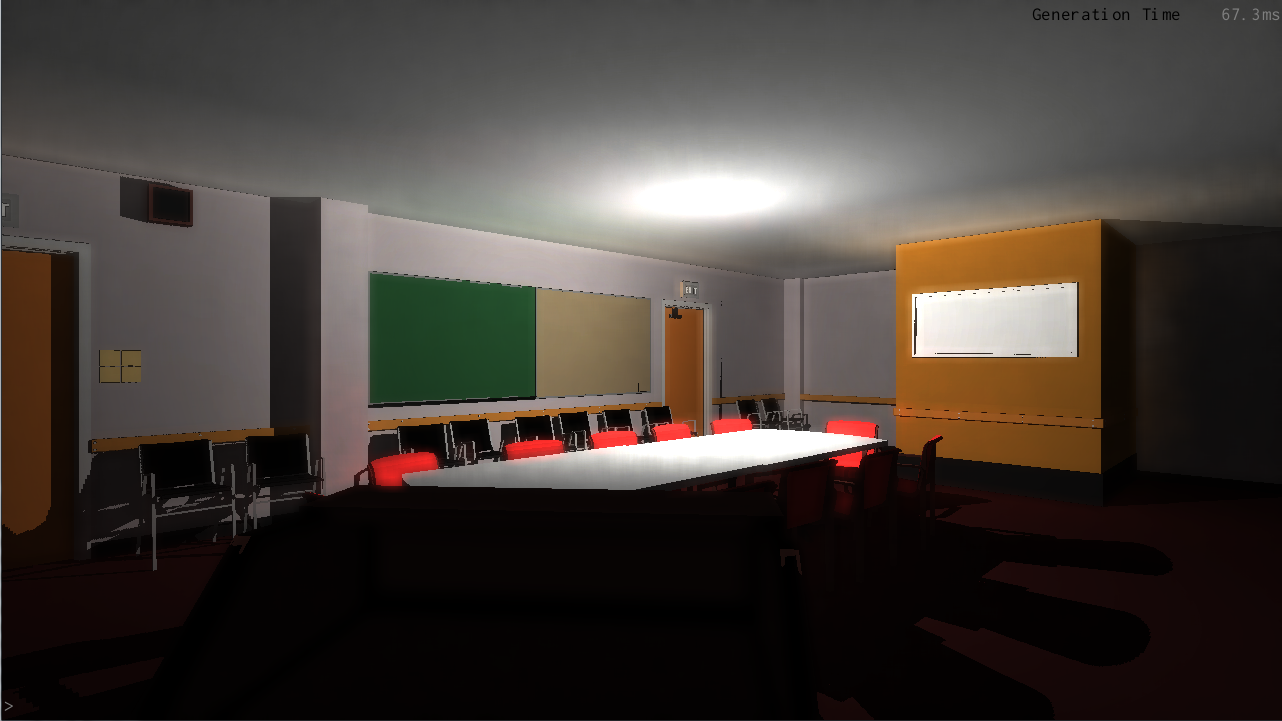
\includegraphics[scale=0.1,trim=0 0 0 -5]{img/results/composite/conference-1layer} \\
\hline
\emph{Frame Time} & 35.0ms & 43.0ms & 67.3ms\\
\hline
\multicolumn{4}{|c|}{\emph{Two Layers}} \\
\hline
\emph{Rendering} &
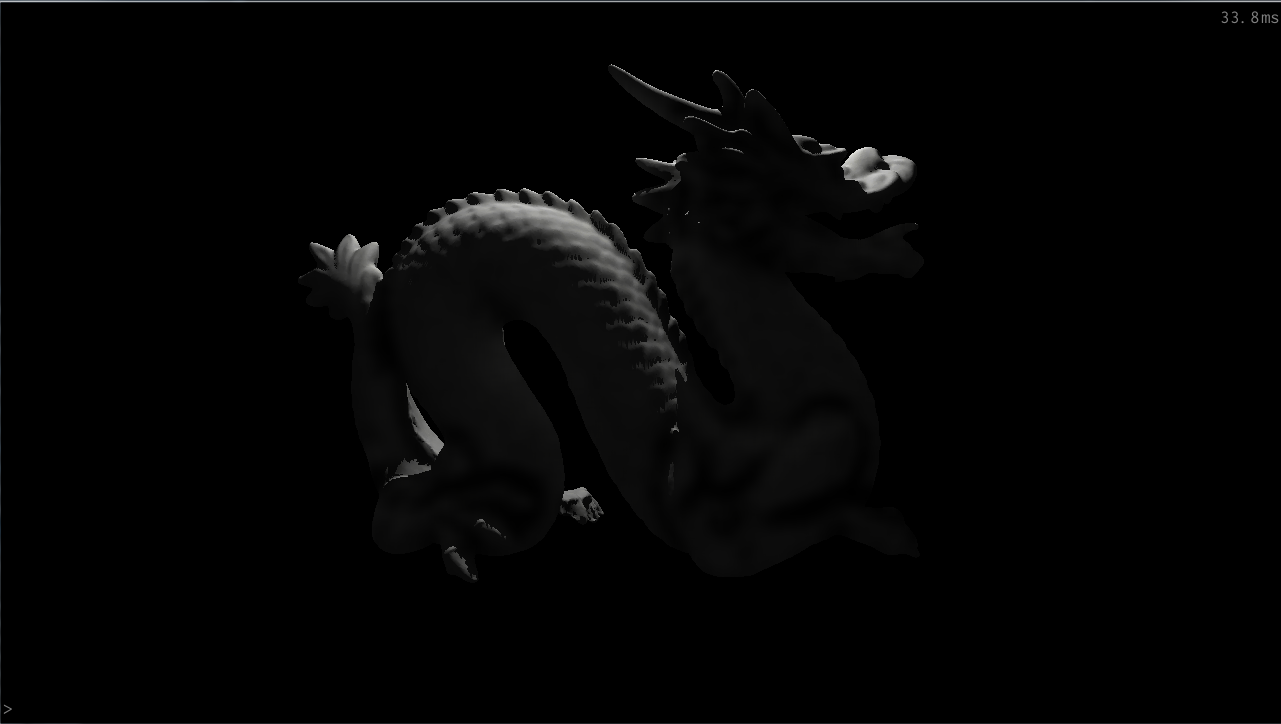
\includegraphics[scale=0.1,trim=0 0 0 -5]{img/results/composite/dragon-2layer} &
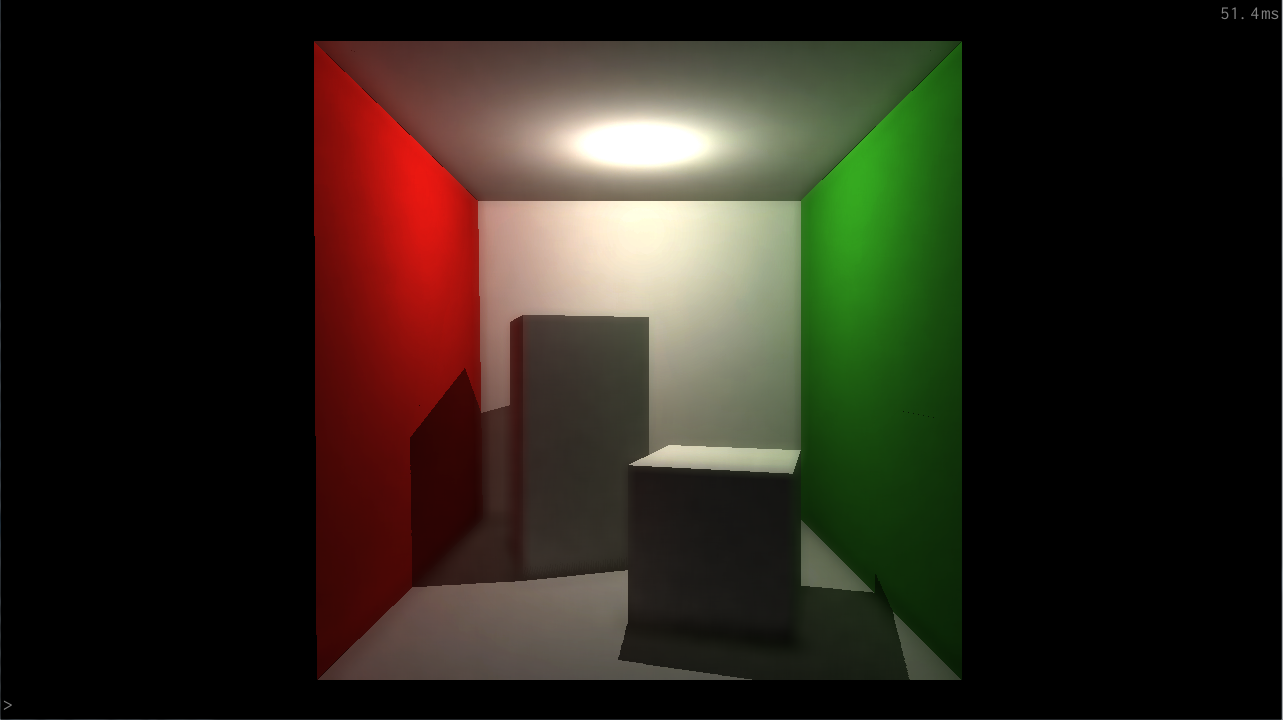
\includegraphics[scale=0.1,trim=0 0 0 -5]{img/results/composite/cornell-2layers} &
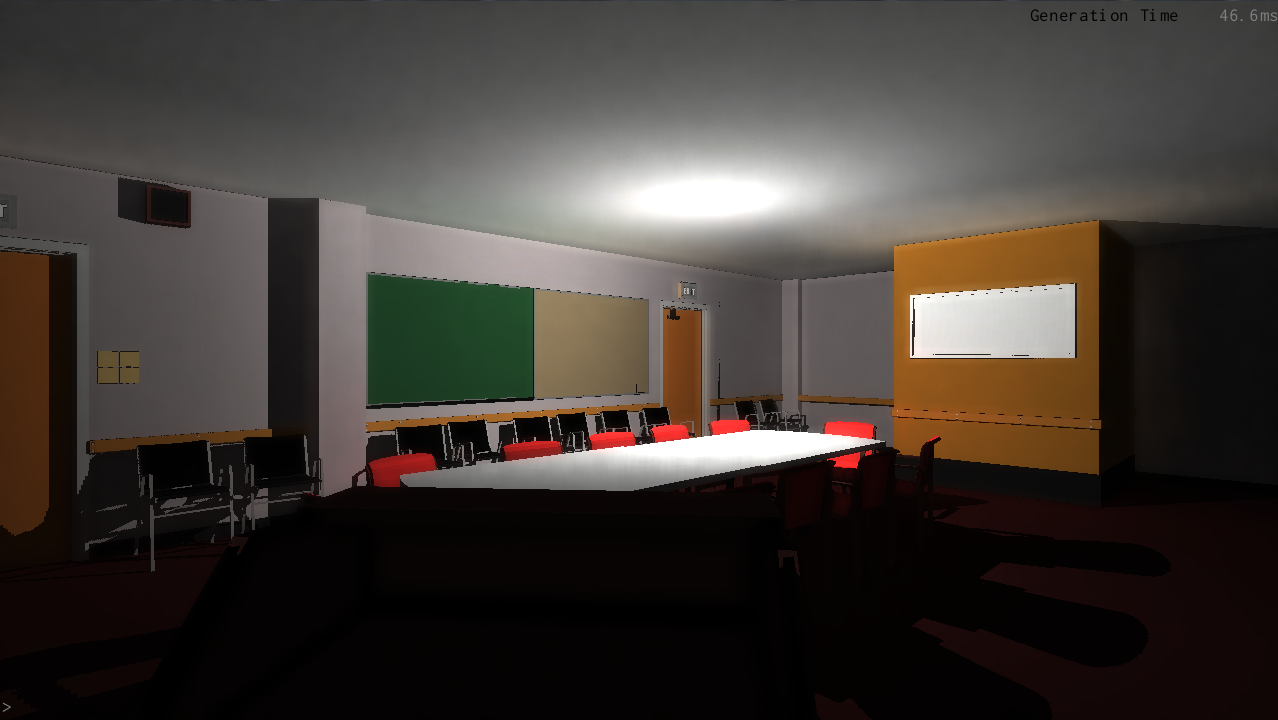
\includegraphics[scale=0.1,trim=0 0 0 -5]{img/results/composite/conference-2layer} \\
\hline
\emph{Frame Time} & 55.6ms & 51.4ms & 50.6ms\\
\hline
\end{tabular}
\caption{Time to draw the final scene with one or two layers of G-buffer. Samples = 23, Radiosity bounces = 1.}
\label{table-final}
\end{center}
\end{table}

\subsection{Discussion}
My first thought here is that there's no noticeable difference between one-layered and two-layered rendering in terms of the final output. There are some minor differences, where you can see some slight contribution from a surface hiding behind another. This is primarily caused, however, by the choice in scenes. These are all geometrically simple scenes, in the sense that there isn't a lot of geometric variation. This also means that the purpose of the deep G-buffer is lost. \ref{table-provingapoint} demonstrates one case in which the deep G-buffer is an advantage, since you can see green contribution on the ceiling from the chalkboard occluded by the chair. That in mind, however, the advantages presented by the deep G-buffer do not, in my opinion, justify the additional costs documented throughout this chapter. Luckily, however, there are multiple ways in which to improve performance. First of all, changing the shadow-map to a cheaper method with two planes in stead of one using dual paraboloid shadow mapping. Secondly, changing the radiosity render targets to a more efficient format and looking for other reasons why it might run that much slower than the SSAO filter. It would also be an option to look into the gaussian filter to maybe only sample every other fragment in the source texture, to cover the same area with less samples, at the cost of filtering quality. Obviously, it would be a good idea to look into the G-buffer generation to figure out why the single-pass generation still doubled the generation time, since it would be an ideal place to look for performance improvements.

\begin{table}[!ht]
\begin{center}
\begin{tabular}{| c | p{5cm} | p{5cm} |}
\hline
&
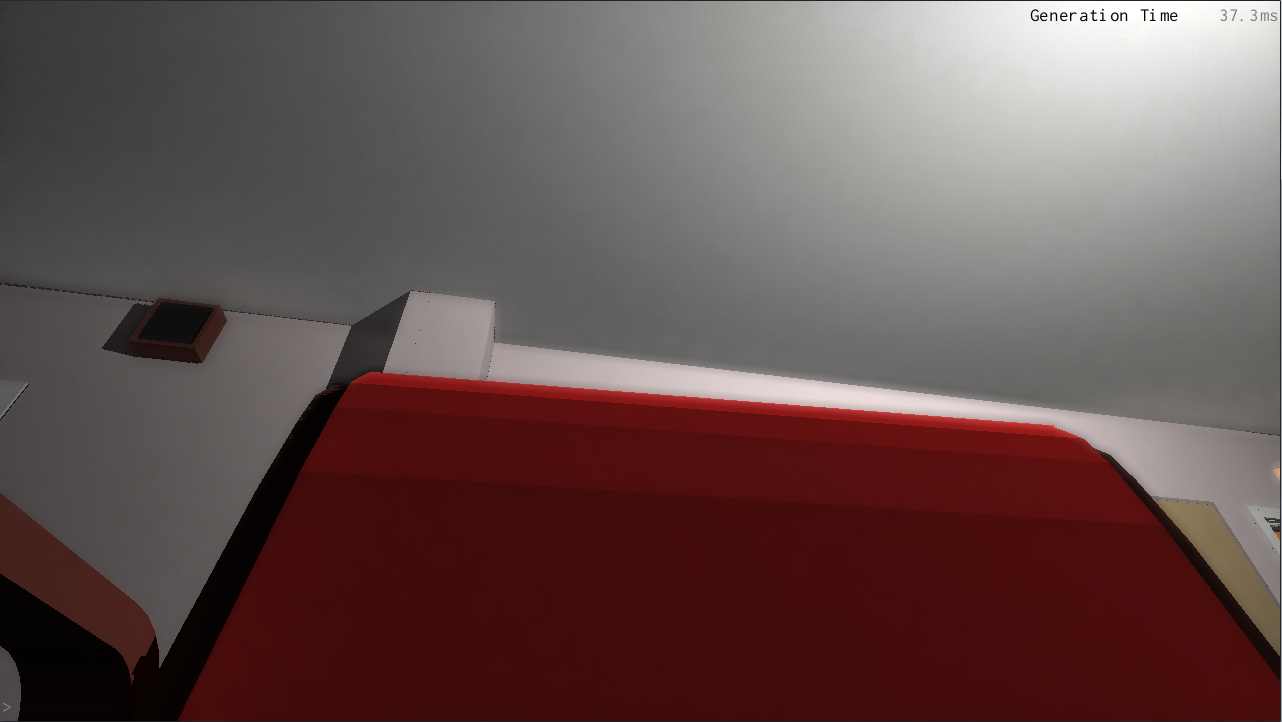
\includegraphics[scale=0.15,trim=0 0 0 -5]{img//results/various/1layer-rad} &
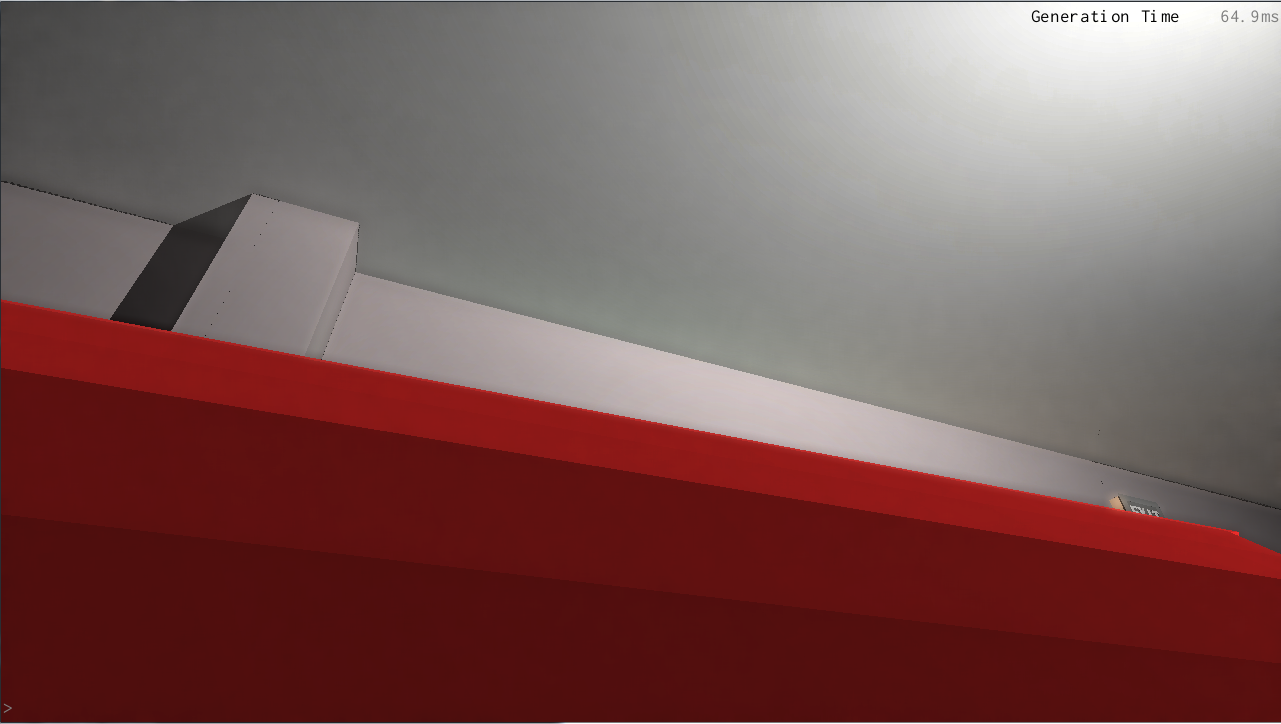
\includegraphics[scale=0.15,trim=0 0 0 -5]{img/results/various/2layer-rad} \\
\hline
\emph{Layers} & 1 & 2 \\
\hline
\end{tabular}
\caption{Demonstrating advantage of deep G-buffer.}
\label{table-provingapoint}
\end{center}
\end{table}

In general, the final product of this thesis demonstrated the concepts of screen-space radiosity, recostruction of positions from a depth buffer, SSAO and omni-directional shadow mapping, it failed to prove the advantage of a deep G-buffer. The costs of it, both in terms of memory and performance, simply turned out to not be worth the benefit. However, a lot of the problems appear to be fixable with optimisations, and I would consider it a reasonable claim that with optimisations and temporal filtering for multiple radiosity bounces, it would be possible to get very reasonable frame times. We're already very close to frame-times that would be considered acceptable for interactive applications, 50ms or 20FPS. Also, the conclusion that I did not prove the usefulness of a deep G-buffer is also influenced by the choice in scenes; different scenes may lead to other conclusions. Of course, the pipeline still has the problem that anything that escapes the viewing frustum will lose its impact on the scene, which is a problem that will persist regardless of scene due to the nature of deferred rendering.